\documentclass{slides}
%
%babel
\usepackage[romanian]{babel}
%
\usepackage{graphicx}%dorim să importăm grafică
\usepackage{amsfonts}
\title{Legile lui Newton}
\author{Pleantă Mihai-Alexandru\footnote{313AC}}
\date{}
\begin{document}
\maketitle
%\begin{abstract}
\textbf{Lucrarea prezintă elemente introductive privind legile lui Newton}
%\end{abstract}
%
%\section{Introducere}\label{intro}
\begin{center}
\textbf{Introducere}
\end{center}
Legile lui Newton (sau principiile fundamentale ale mecanicii) sunt trei legi ale fizicii care dau o relație directă între forțele care acționează asupra unui corp și mișcarea acelui corp. Ele au fost enunțate de Sir Isaac Newton (bazat și pe studiile lui Galilei) în lucrarea sa Philosophiae Naturalis Principia Mathematica (1687). Aceste legi formează baza mecanicii clasice.
%\section{Tratare}
\begin{center}
\textbf{Principiul al II-lea al mecanicii}
\end{center}
Principiul al II-lea al mecanicii: Newton a descoperit faptul că o forță care acționează asupra unui corp îi imprimă acestuia o accelerație, proporțională cu forța și invers proporțională cu masa corpului:
\begin{equation}
\vec{F}=m\vec{a}
\end{equation}
Urmează tabelul de definire a unităților de măsură a componentelor principiului forței
%\begin{table}[htbp]
\centering
%\caption{Unități de măsura}\label{tab:unit}
\begin{tabular}{lll}
\hline
Nr.&Mărime&Unitate de măsură\\\hline
1&masa&[kg]\\\hline
2&accelerația&[m/$s^2$]\\\hline
3&forța&[(kg*m)/$s^2$]
\end{tabular}
%\end{table}
%\begin{figure}[ht]
\centering
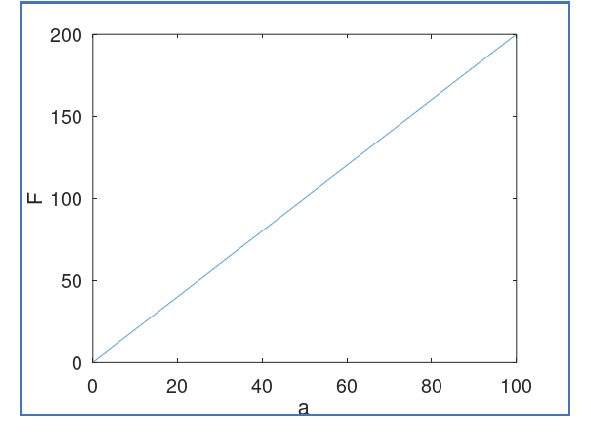
\includegraphics[scale=0.8]{figura.pdf}
%\caption{Evoluția ...}
%\end{figure}
%\section{Concluzii}
\begin{center}
\textbf{Concluzii}
\begin{center}

\end{center}
\end{center}
%\begin{thebibliography}{a}
%\bibitem{wiki} Wikipedia-Legile lui Newton: \verb+https://ro.wikipedia.org/wiki/Legile_lui_Newton+
%\end{thebibliography}
\end{document}